\section{问题重述}

无线电干扰源的精准定位与清除，是频谱管理链条中最耗时、也最依赖现场经验的一段。题面将前期大范围监测已经完成的结果抽象为一个半径 $1800\,\mathrm{m}$ 的圆域 $\Omega$，并以圆心为原点、正东为 $x$ 轴、正北为 $y$ 轴建立平面直角坐标系。方位角从正东逆时针计量，取值于 $[0^\circ,360^\circ)$。圆域内有未知个数的干扰源，每个源占用互不相同且时不变的频道；频道编号取自常见的 $20$ 个频道，并不存在“二十个频道上都有源”的隐含假设。待研发的系统把测向机、简易光学探测仪与激光清除装置搭载在机器狗上，以代替技术人员进入危险环境完成精准定位与清除。

测向机一次只能检测一个频道。机器狗必须先停止移动，必要时花费 $1\,\mathrm{s}$ 切换频道，再花费 $5\,\mathrm{s}$ 调整天线并读出示向度或确认无信号。示向度是检测点指向源的方位角，读数相对真方位的误差落在闭区间 $[-1^\circ,1^\circ]$，接口保留两位小数；同一地点、同一频道的误差不因重复检测而独立刷新，因而重复测量仍支付虚拟时间，却不能当作新的独立样本。当检测点落入源的有效覆盖且距离不超过 $5\,\mathrm{m}$ 时，场强过强，接口不再返回角度，只能直接启用光学精确定位，不得把缺失的角度填成 $0^\circ$。光学定位成功的几何条件是欧氏距离不超过 $20\,\mathrm{m}$，与射频朝向无关；光学耗时 $3\,\mathrm{s}$，激光清除成功再加 $2\,\mathrm{s}$，失败仍支付光学时间。机器狗沿直线以 $5\,\mathrm{m/s}$ 行进，坐标分量绝对值不得超过 $2\times 10^6\,\mathrm{m}$，但允许走出圆域 $\Omega$——$\Omega$ 只约束源的位置，圆外测点是给贴边朝外的定向源准备的，不是把源放到圆外。

按辐射角度，源分为全向源与定向源。
全向源在 $360^\circ$ 内均匀辐射；定向源的有效覆盖是其定向方向两侧各 $90^\circ$（含）的闭扇，总宽 $180^\circ$。
各源的有效接收半径 $r_i$ 落在 $[1000,1500]\,\mathrm{m}$，对机器狗不可观测。
覆盖判定使用源指向检测点的方向，示向度则是检测点指向源，二者相差 $180^\circ$。
接口不提供场强或距离，不能做距离回归。
定向扇外即使欧氏距离很小也可能测不到射频，但光学清除仍只检查 $20\,\mathrm{m}$，因此问题4必须把发现证书与清除证书分开，而不能把无信号读成距离圆盘。
圆域只约束源位，机器狗出圆是给贴边朝外的定向源准备测点，不是把源放到圆外。

计时上必须区分三套时钟，不得混用。虚拟任务时间 $T$ 计入移动、切换、检测、光学与成功激光，空扫与失败动作同样计费，上限 $360000\,\mathrm{s}$；效率指标为平均定位清除时间 $T/K$，其中 $K$ 为成功清除个数，$K=0$ 时该比值未定义，应留空而不是填零。程序运行时间是从 $\mathtt{/enter}$ 到结束的墙钟，上限 $1200\,\mathrm{s}$，对应表1第四列。测试窗口另有 $1500\,\mathrm{s}$。$\mathtt{/enter}$ 与 $\mathtt{/exit}$ 不推进虚拟时间；被拒绝的指令不得覆盖时钟。倒计时 $5\,\mathrm{s}$ 内接口未开放。正式测试与演练测试的物理环境一致，但正式测试每问独立三次额度、中止也占次，且永不返回源的总数 $N$；演练结束可得到 $N$，仅用于核对 $K/N$，不能写入正式成绩表。截止时间 $2026$ 年 $9$ 月 $13$ 日 $17$:$30$（北京时间）之后不能启动新的正式测试。题面与附件冻结的动作耗时与几何常数见表~\ref{tab:params}，后文求解器不另写一套常数。

\begin{table}[H]
\centering
\caption{冻结动作与几何常数}
\label{tab:params}
\begin{tabular}{lccl}
\hline
量 & 数值 & 单位 & 口径 \\
\hline
目标圆域半径 & $1800$ & $\mathrm{m}$ & 只约束源位 \\
源数上下界 & $10$--$16$ & 个 & 在线未知 \\
频道编号 & $1$--$20$ & --- & 每频道至多一源 \\
接收半径 & $1000$--$1500$ & $\mathrm{m}$ & 接口不返回 \\
示向度误差 & $\pm 1$ & $^\circ$ & 闭区间，同点不刷新 \\
近区 / 光学半径 & $5$ / $20$ & $\mathrm{m}$ & 闭边界 \\
行进速度 & $5$ & $\mathrm{m/s}$ & 直线 \\
检测 / 切换 & $5$ / $1$ & $\mathrm{s}$ & 空扫同样计费 \\
光学 / 成功激光 & $3$ / $2$ & $\mathrm{s}$ & 失败仍付光学 \\
墙钟 / 窗口 / 虚拟上限 & $1200$ / $1500$ / $360000$ & $\mathrm{s}$ & 三套时钟 \\
正式额度 & $3$ & 次/问 & 中止占次 \\
\hline
\end{tabular}

\vspace{0.4em}
{\small 来源为题面与附件冻结参数表，共 $28$ 项；表中只列后文反复用到的子集。数值包络 $1.005^\circ$ 不列入。}
\end{table}

三套时钟一旦混用，表1第四列就会被虚拟 $T$ 污染，或者把墙钟误当成单位清除时间。
检测 $5\,\mathrm{s}$ 对 $\mathtt{direction}$、$\mathtt{near}$ 与 $\mathtt{no\_signal}$ 同样收取，因此空扫很多频道会直接抬高 $T$，而不能靠事后把无信号从账本里删掉。
光学失败仍支付 $3\,\mathrm{s}$，所以试清点必须有覆盖含义：在连续候选区外盲打，既不能证明该区搜完，还要为失败付费。
这些计时规则在问题3、问题4里不再重复推导，只作为证书层与启发式层的共同约束。
正式额度每问三次、中止占次，写作时两次正式测试均未启动，后文成绩表保持空缺。

问题1在若干检测点及其示向度已知时，要求给出交会定位多边形直径的算法，并判断以该直径为直径的圆能否覆盖定位区域。问题2只给出一个全向源在一个检测点上的示向度，要求给出第二个检测点的选择策略及其候选区域。问题3假设全部为全向源，总数 $N\in\{10,\ldots,16\}$ 在线未知，机器狗从原点出发、初始频道为 $1$，在保证全部清除的前提下尽量缩短任务时间；须按表1报告三次正式测试。问题4在问题3的基础上引入未知个数与未知朝向的定向源，其余协议、计时与正式测试额度均独立继承。两问的字典序目标都是先保证 $K=N$，再尽量缩短 $T$；由于正式测试不返回 $N$，在线策略不能把“已经清除 $10$ 个”写成结束条件，也不能用单点二十频道无信号代替频道判空。

全文按“几何交会 $\to$ 第二测点 $\to$ 全向在线清除 $\to$ 混合源覆盖证书”展开。技术路线把四问的输入、核心对象与输出串在同一张图上，后文各问只展开对应流程，不再重复总览。

\begin{figure}[H]
\centering
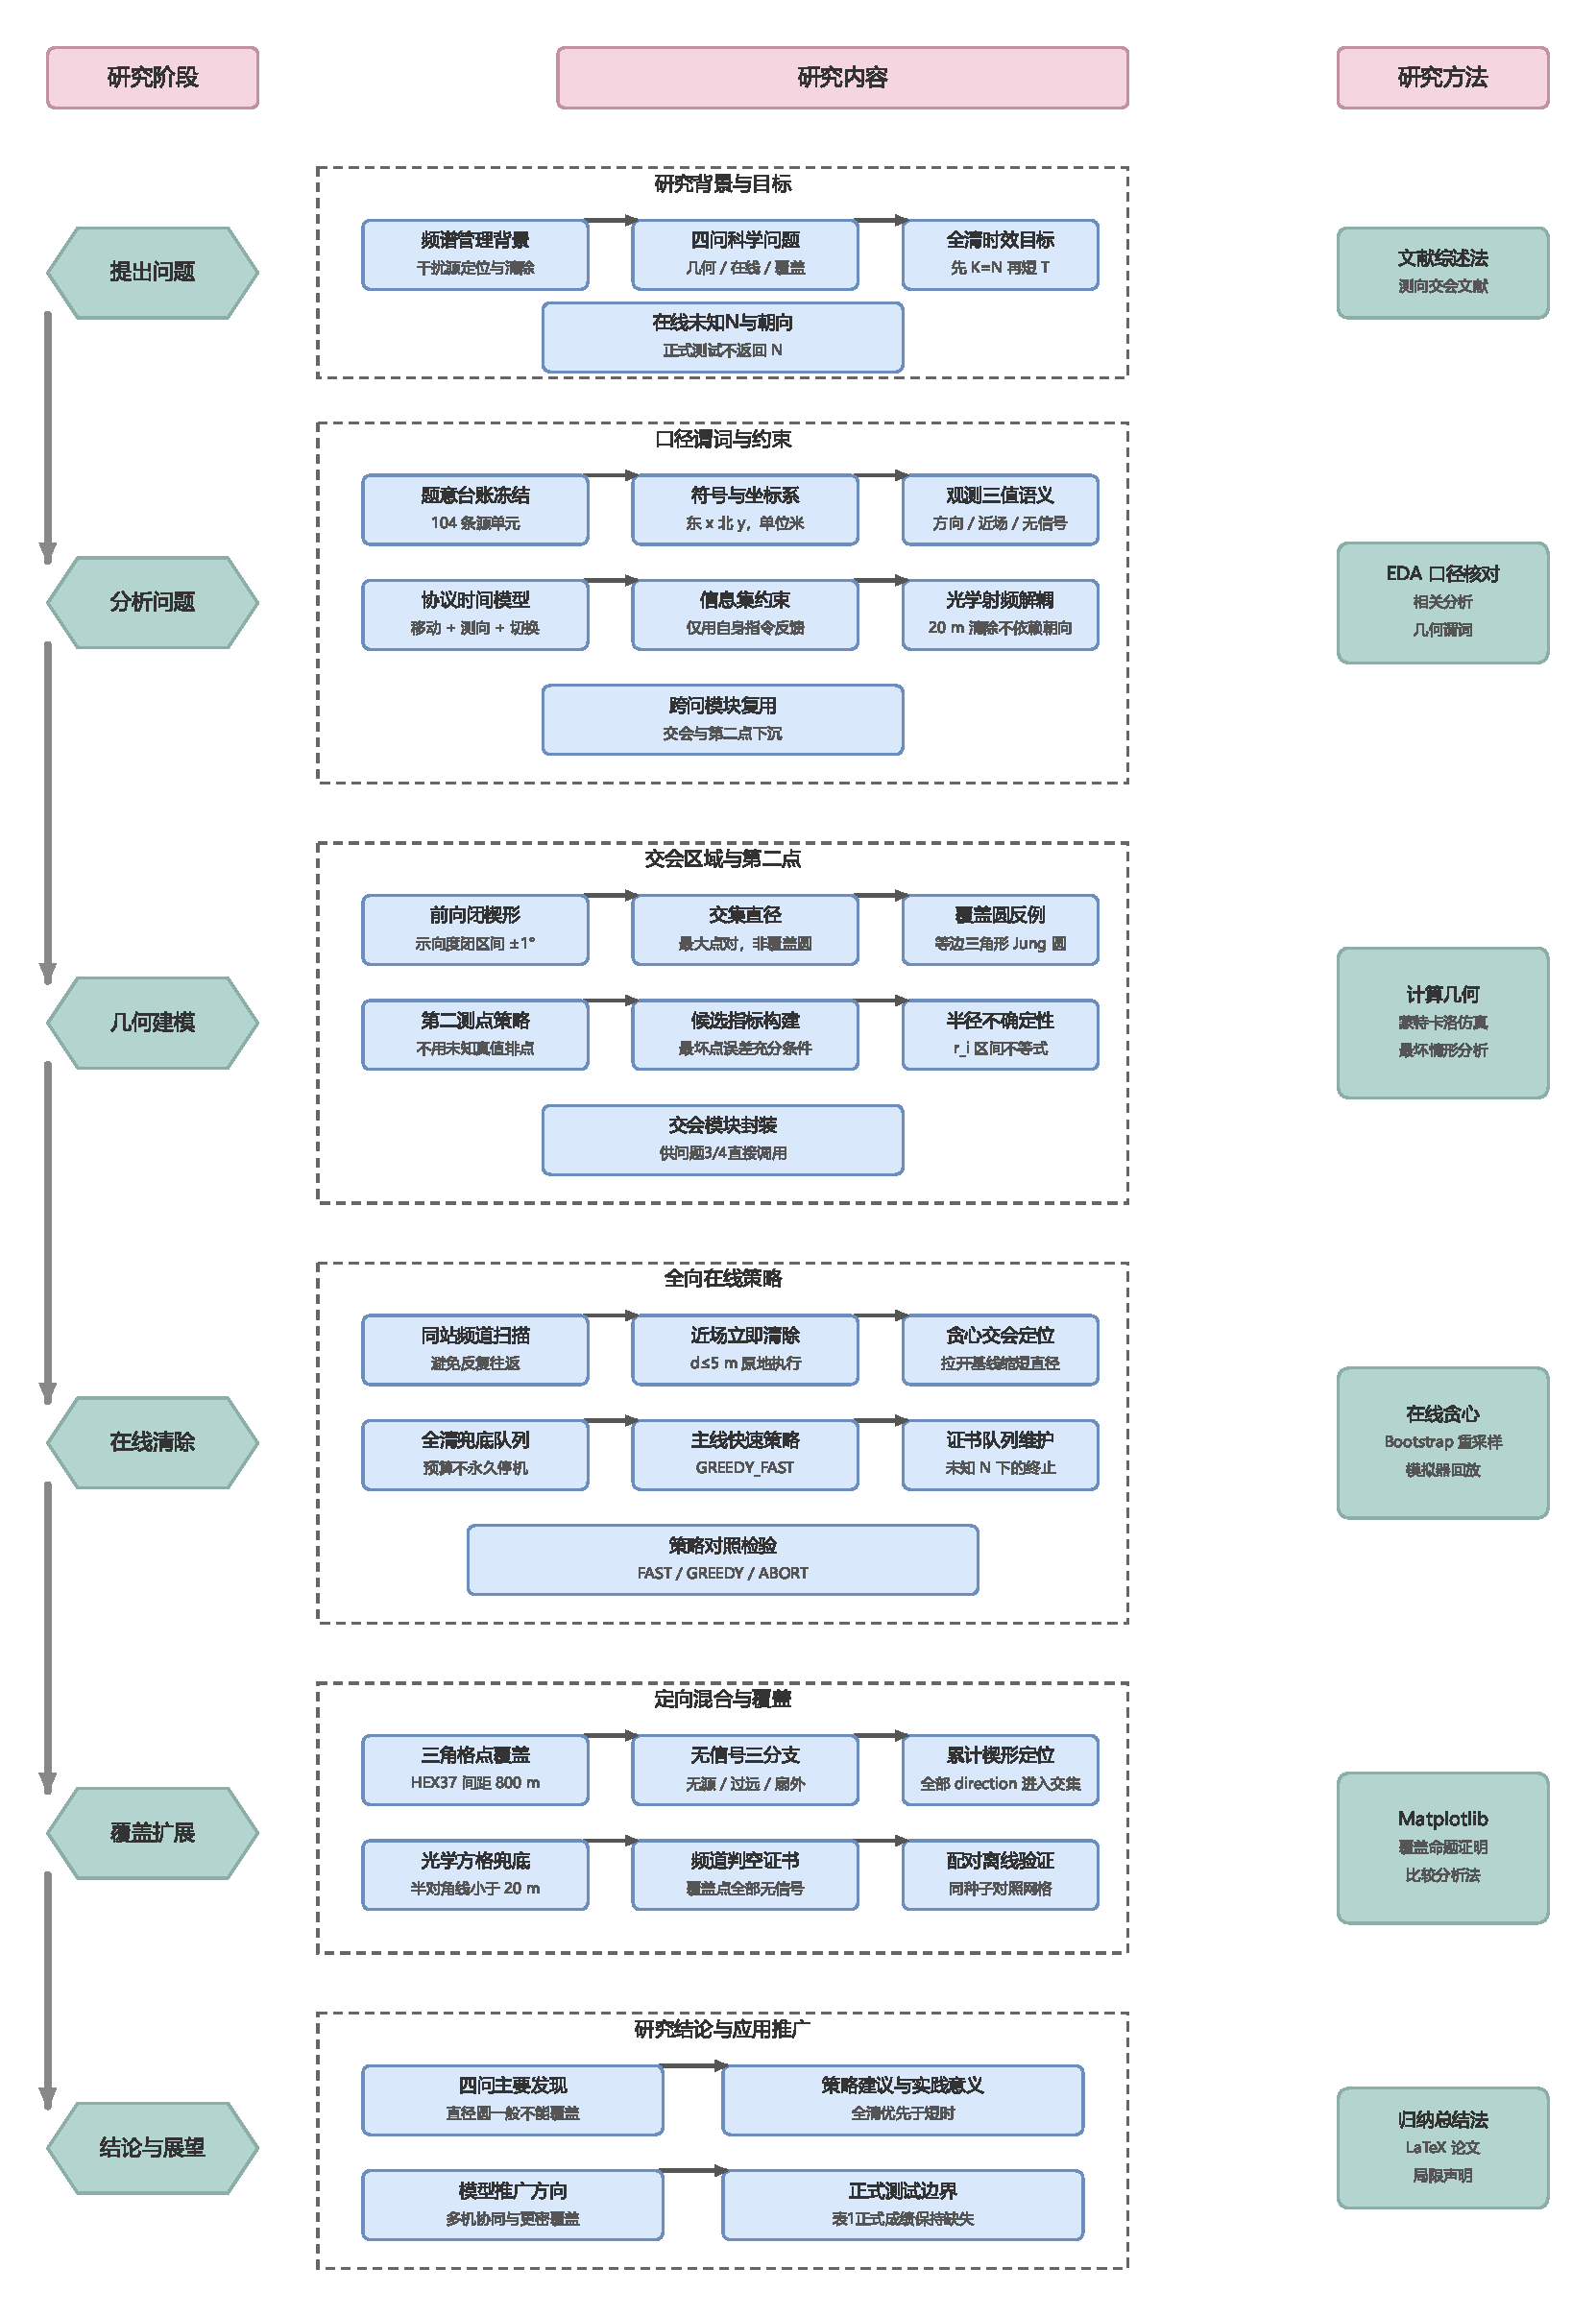
\includegraphics[width=\textwidth,height=0.62\textheight,keepaspectratio]{../figures/fig_roadmap.pdf}
\caption{技术路线总览}
\label{fig:roadmap}
\end{figure}

四问共用同一套观测与动作，但完备性证书并不共用。
问题1交付的是楔形交集上的直径与覆盖判定，并不假设定位区有界非空。
问题2在单次示向度外包络上推荐第二点，排序指标不是清除证书。
问题3用原点加半径 $1200\,\mathrm{m}$ 的正六边形七点做发现巡回，主线策略 GREEDY\_FAST 把启发式预算从停机条件上拿掉。
问题4必须改用能同时进入最小接收半径与 $180^\circ$ 开半平面的有限格点，正方形网格 SQUARE81 与三角晶格 HEX37 各有一条覆盖命题，在线求解器再累计全部正向观测并用边长 $28\,\mathrm{m}$ 的光学方格覆盖连续候选区。
路线图只标出这条分层，具体不等式与数字在对应章节给出。

需要预先强调两处容易写错的交付物。其一，本文写作时问题3、问题4的正式测试均尚未执行，表1相应单元格保持空缺，不以演练或离线几何模型的数字填入；支撑材料中的日志若存在，只来自演练模块。其二，$T/K$ 与墙钟不是同一列，$K=0$ 时 $T/K$ 未定义；后文凡引用非正式演练或离线配对的均值，均在表注或正文中标明口径，禁止改名充当正式成绩。
非正式口径下已经冻结、但不得写入表1的数字包括：问题3主线十局平均 $341\,\mathrm{s}$，问题4离线配对 HEX37 的 $836.91\,\mathrm{s}$，PREFIX\_A 离线均值 $683.09\,\mathrm{s}$，以及 PREFIX\_A 演练两场 $822.38\,\mathrm{s}$ 与 $930.28\,\mathrm{s}$。
这四组数字分属演练与离线几何模型，禁止平均成一个现场成绩。
参数表共 $28$ 项，后文求解器不另写一套常数；数值包络 $1.005^\circ$ 只作为量化约定出现在后问实现里，不列入该表。

四问的输入规模也不同。问题1的检测点集由题面给定，输出是算法而不是某一组数字。问题2只有一次示向度，候选区域必须在未知 $g$ 与未知 $r_i$ 下可计算。问题3、问题4的源数在 $10$ 与 $16$ 之间，频道至多 $20$ 个，机器狗从原点、频道 $1$ 出发；正式测试不返回 $N$，在线停机只能依赖频道状态机：每个频道为已清除或证书缺席。后文不再把“大约十个源”写成目标。路线图中的箭头表示依赖：没有楔形交就不会有第二点外包，没有第二点几何就没有发现后的局部测向，没有发现网格就没有判空，没有判空就不能声称 $K=N$。
动作账本按接口计费：检测对三值反馈同样收取 $5\,\mathrm{s}$，切换只在频道改变时收取 $1\,\mathrm{s}$，光学失败仍收取 $3\,\mathrm{s}$，只有成功激光再加 $2\,\mathrm{s}$。
因此空扫很多频道会直接抬高 $T$，试清点必须有覆盖含义，而不能在连续候选区外盲打。
机器狗坐标分量绝对值不得超过 $2\times 10^6\,\mathrm{m}$，越界点直接丢弃；圆域只约束源位，出圆测点是给贴边朝外的定向源准备的。
正式测试与演练的物理环境一致，但正式永不返回 $N$，每问独立三次额度、中止占次，截止之后不能启动新测试。
这套约束在后文各问不再重复推导，只作为证书层与启发式层的共同边界。
